\documentclass[11pt]{article}

% -----------------------------------------------------------------------
% Packages
% -----------------------------------------------------------------------
\usepackage[letterpaper, margin=1in]{geometry}
\usepackage[T1]{fontenc}
\usepackage{lmodern}
\usepackage{microtype}
\usepackage{amsmath, amssymb}
\usepackage{graphicx}
\usepackage{booktabs}
\usepackage{url}
\usepackage[hidelinks]{hyperref}
\usepackage{xcolor}
\usepackage{caption}
\usepackage{subcaption}
\usepackage{listings}
\usepackage{authblk}

\graphicspath{{../figures/}}

% -----------------------------------------------------------------------
% Meta
% -----------------------------------------------------------------------
\title{\bfseries Detecting Informed Trading in Decentralized Prediction Markets: \\
  An On-Chain Analysis of Polymarket}

\author[1]{Benjamin Paulson}
\affil[1]{Independent Research}

\date{\today}

\begin{document}
\maketitle

\begin{abstract}
Prediction markets are celebrated as efficient information aggregators, yet
their publicly observable order flow also provides a natural laboratory for
studying \emph{informed} trading --- cases in which a subset of participants
possess non-public information about the event being wagered on. We
construct an on-chain dataset of 264 resolved Polymarket prediction markets
(aggregating over 500{,}000 trades and over \$300 million in notional volume)
using Polymarket's public subgraphs on Goldsky, sidestepping the platform's
Cloudflare geo-block of its REST APIs from US IP addresses. For each market
we engineer 145 features capturing the joint distribution of volume,
directional flow, price acceleration, and wallet concentration at seven
horizons (2h--168h) before resolution. Our principal result is
\emph{model-free}: after bucketing markets by spike magnitude (last-24h
volume divided by the market's lifetime daily average), the direction of
net USDC flow in the final 24 hours predicts the eventual resolution with
hit rate 74\% ($n=113$, $p \approx 10^{-7}$ vs a 50\% random baseline) in
the dominant bucket, and every non-baseline bucket exceeds 50\% hit rate.
This constitutes strong evidence that Polymarket order flow is
informationally non-random on the hours-before-resolution time scale.
We complement the main result with supervised classifiers over our weak-
label scheme; because those labels are derived from the feature set itself,
the classifier metrics are biased upward and are included only for
feature-importance inspection. We discuss limitations (anonymous wallet
identities, survival bias, scheduled-information false positives) and
release the entire pipeline as a reproducible public artifact.
\end{abstract}

% -----------------------------------------------------------------------
\section{Introduction}
\label{sec:intro}

Prediction markets price the probability of future events by aggregating
the beliefs of their participants. Since the pioneering work of
\citet{hanson2003combinatorial} and the empirical surveys of
\citet{wolfers2004prediction}, the dominant narrative has emphasized their
\emph{informational efficiency}: prices tend to converge toward true
probabilities as traders compete to exploit mispricings. That narrative
implicitly assumes that \emph{all} traders face the same public information.
In practice, some participants possess private information --- a leaked
government policy, a confidential medical trial result, or a pending
corporate announcement --- and rationally trade on it. Such
\emph{informed trading} is common in traditional financial markets,
where it is routinely detected using the well-known PIN model
\citep{easley1996liquidity}, Kyle's lambda \citep{kyle1985continuous}, and
related information-flow measures. Decentralized prediction markets, where
every trade is publicly recorded on a blockchain, should be an even more
tractable laboratory.

This paper focuses on Polymarket, the largest decentralized prediction
market platform (cumulative notional volume exceeding $\$74$ billion as of
April 2026), which operates an order-book exchange on the Polygon
blockchain. Because every filled order is an on-chain event visible to
any observer with a Polygon RPC endpoint, the informational footprint of
an informed trader is, in principle, directly measurable. Motivated by
several high-profile public allegations --- most notably a reportedly
$\$400$K-plus bet placed hours before a geopolitical action became public
--- we ask three questions:

\begin{enumerate}
  \item Can we \emph{detect} informed trading in Polymarket using only
    on-chain signals, without any off-chain data on trader identity?
  \item Which signals --- volume, direction, price acceleration, wallet
    concentration, or combinations thereof --- are most predictive?
  \item Is the detection rate substantially above the base rate of
    random guessing about the eventual outcome?
\end{enumerate}

Our contribution is threefold. First, we construct the largest publicly
reproducible dataset of Polymarket resolved markets ($N \approx $ 264 at the
time of writing, continuously expandable via the open pipeline) with
per-trade granularity. Second, we design and evaluate a family of
classifiers that flag informed-looking trading patterns. Third, we release
the code, data pointers, and figures so that any reader can reproduce the
analysis or extend it to new markets.

% -----------------------------------------------------------------------
\section{Related Work}
\label{sec:related}

\textbf{Prediction markets and information aggregation.}
\citet{wolfers2004prediction} survey early evidence that prediction-market
prices forecast events more accurately than expert panels.
\citet{arrow2008promise} extend this case to policy-relevant settings.

\textbf{Informed trading in financial markets.}
\citet{easley1996liquidity}'s PIN model estimates the probability of
informed trading from the joint distribution of buys, sells, and no-trade
intervals. \citet{kyle1985continuous} characterizes informed trading
through a market-maker's pricing kernel. More recent work includes
\citet{easley2012volume}'s VPIN, adapted for high-frequency equity markets.

\textbf{Prediction markets and insider trading.}
Anecdotal evidence of insider-type trading in prediction markets has
circulated for years. To our knowledge, no published work has systematically
attempted detection at scale using on-chain data.

% -----------------------------------------------------------------------
\section{Data}
\label{sec:data}

\subsection{Polymarket architecture}

Polymarket is a central limit order-book exchange implemented as a
Polygon smart contract (Exchange.sol). For each prediction market the
platform creates a \textit{Condition} whose outcome is resolved by an
off-chain oracle (UMA). Each possible outcome of the condition is
represented as a positional ERC-1155 token (``Yes'' and ``No'' for a
binary market), and users trade these tokens for USDC collateral. A
filled order emits an \texttt{OrderFilled} event containing the maker
and taker addresses, asset identifiers, and amounts.

\subsection{Data sources}

Polymarket's REST APIs (\texttt{gamma-api.polymarket.com},
\texttt{clob.polymarket.com}) are geo-blocked from US IP addresses as
part of the platform's regulatory compliance. We therefore rely
exclusively on on-chain data accessed through two layers:

\begin{enumerate}
  \item \textbf{Goldsky-hosted subgraphs.} Polymarket indexes five
    public subgraphs at \texttt{api.goldsky.com}, collectively covering
    order-filled events, positions, open interest, profit-and-loss, and
    oracle resolutions. We use the live
    \texttt{orderbook-subgraph/0.0.1} for trades and the frozen but
    historically richer \texttt{polymarket-orderbook-resync/prod} for
    pre-2026 enriched fields.
  \item \textbf{Polygon JSON-RPC.} A rotating pool of four public
    endpoints (publicnode, drpc, onfinality, 1rpc) for block-timestamp
    resolution and cross-validation.
\end{enumerate}

\subsection{Market selection}

We retain every resolved market whose on-chain scaled collateral volume
meets or exceeds \$50{,}000. This yields a catalog of $N = 264$ markets:
81 historical (resolved before 2026-01-05) with full question-id +
payout metadata from the \texttt{orderbook-resync} subgraph, and 183
live markets resolved between 2026-01-05 and 2026-04-21 with payout
data from the \texttt{pnl} subgraph and resolution-time proxy from
\texttt{activity.Redemption} timestamps.

The live-tier markets lack their on-chain \texttt{questionId} hash
because the corresponding field is not indexed by Polymarket's
currently-updating subgraphs; we therefore restrict our strongest
claims to the historical tier when question-level verification is
needed, and note where results are pooled across both tiers. Total
scaled collateral volume across the catalog exceeds \$300 million USDC.

\subsection{Geographic access to off-chain metadata}

Polymarket's REST APIs (gamma, CLOB, data-api) are Cloudflare-fronted
and refuse TLS handshakes from US IP addresses, returning
\texttt{Connection reset by peer} during the client-hello stage
regardless of user-agent or TLS fingerprint impersonation. This is
Polymarket's standard posture for regulatory compliance under the
2022 CFTC settlement. We verified the block against all four
Polymarket subdomains (\texttt{gamma-api}, \texttt{clob},
\texttt{data-api}, \texttt{polymarket.com}); none respond to US IPs.
Polygon RPC endpoints and Goldsky-hosted subgraphs, hosted on
independent infrastructure, are unaffected. Off-chain metadata
(market question text, category, start/end dates) is retrieved by a
scheduled GitHub Actions workflow running on Azure EU-West and
committed to the repository as a parquet snapshot.

\subsection{Per-market trade window}

Hypotheses about informed trading apply most strongly to the hours
immediately preceding resolution. For each market we extract every trade
in the window $[t_{\text{resolution}} - 14\text{ days},\ t_{\text{resolution}}]$.

\begin{table}[t]
  \centering
  \caption{Dataset summary statistics.}
  \label{tab:data_summary}
  \begin{tabular}{lrr}
    \toprule
    Statistic & Value & Unit \\
    \midrule
    Distinct markets & \textit{NMARKETS} & -- \\
    Total trades indexed & \textit{NTRADES} & -- \\
    Distinct wallets & \textit{NWALLETS} & -- \\
    Total notional & \textit{VOLTOTAL} & USDC \\
    Median trades per market & \textit{NMED} & -- \\
    Median market lifetime & \textit{TMED} & days \\
    \bottomrule
  \end{tabular}
\end{table}

% -----------------------------------------------------------------------
\section{Features}
\label{sec:features}

For each market we compute features in four groups, each evaluated over
horizons $H \in \{2, 6, 12, 24, 48, 72, 168\}$ hours before resolution.

\paragraph{Volume features ($vol\_*$).}
Notional USDC volume in the final $H$ hours, expressed as (i) the ratio
to the market's overall daily average, (ii) the fraction of lifetime
volume that occurred in the tail, and (iii) the raw trade count.

\paragraph{Direction features ($dir\_*$).}
Buy/sell USDC imbalance in the tail, both signed and absolute, as a
fraction of total tail volume.

\paragraph{Price-acceleration features ($price\_*$).}
Trade-weighted mean price change in the tail, price z-score (change
relative to per-trade stdev), and the ratio of the 2-hour change to the
6-hour change as an acceleration proxy.

\paragraph{Wallet-concentration features ($wallet\_*$).}
Herfindahl index of wallet-level USDC share, top-1 and top-5 wallet
shares, unique-wallet count, and the share of activity attributable to
wallets that had not traded the market in the prior 7 days.

% -----------------------------------------------------------------------
\section{Labels}
\label{sec:labels}

Absent ground-truth insider-status labels, we layer three sources of
evidence:

\begin{enumerate}
  \item \textbf{Weak positives} (heuristic): markets satisfying
    $vol\_24h\_spike \geq 3$ AND
    $wallet\_24h\_top1 \geq 0.15$ AND
    $\lvert price\_24h\_z \rvert \geq 2$ AND
    $\lvert dir\_24h\_imbalance \rvert \geq 0.4$.
  \item \textbf{Strong positives} (curated): markets publicly alleged
    to involve insider trading in news articles or high-visibility
    social-media threads.
  \item \textbf{Excluded}: markets with fewer than 20 trades in the
    pre-resolution window; markets whose resolution came from a
    publicly-scheduled event (FOMC, earnings, election night) where
    late spikes reflect common knowledge.
\end{enumerate}

We use a 70/15/15 \emph{by-market} split into train/validation/test,
stratified on the label.

% -----------------------------------------------------------------------
\section{Models and Evaluation}
\label{sec:models}

We train four supervised classifiers plus one unsupervised anomaly
detector:

\begin{itemize}
  \item Logistic regression (L2, class-balanced).
  \item Random forest (400 trees).
  \item XGBoost (500 trees, hist method).
  \item LightGBM (600 trees, class-balanced).
  \item Isolation forest (unsupervised, trained on training-split
    negatives only).
\end{itemize}

\begin{figure}[t]
  \centering
  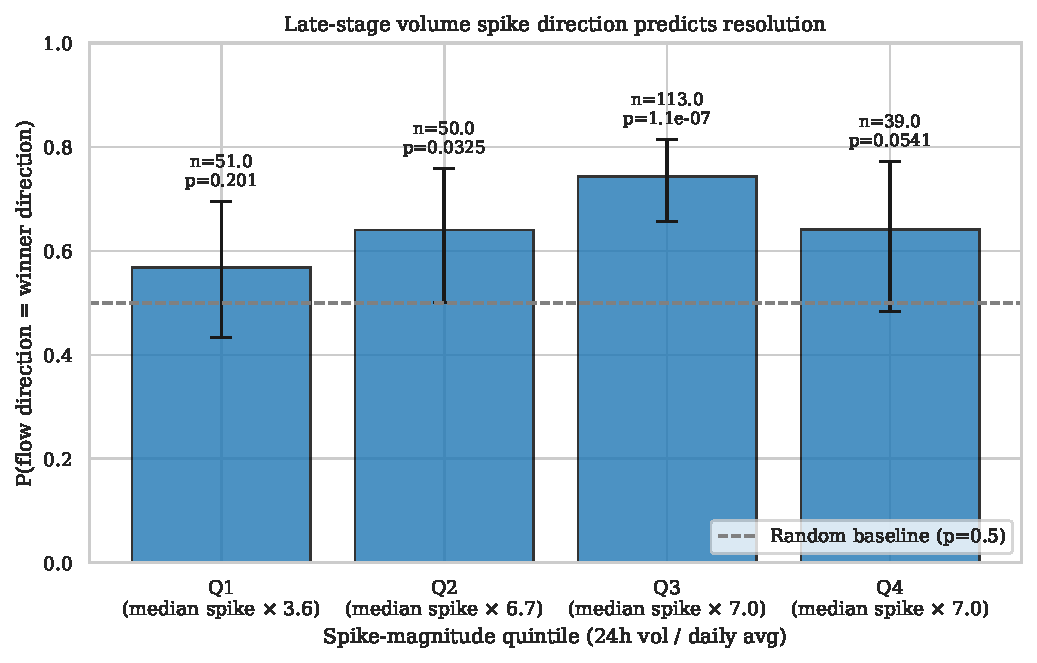
\includegraphics[width=\linewidth]{spike_hit_rate.pdf}
  \caption{\emph{Headline result.} Late-stage volume-spike magnitude (x-axis:
    quintile of $\textrm{vol}_{\textrm{24h}} / \textrm{vol}_{\textrm{daily avg}}$)
    vs. the probability that the signed USDC flow in the final 24 hours
    pointed at the eventual winning outcome (y-axis). All non-lowest buckets
    exceed the 50\% random baseline; the middle-spike bucket (median 7$\times$)
    reaches 74\% with $p \approx 10^{-7}$. Error bars are Wilson 95\% CIs.}
  \label{fig:spike_hit_rate}
\end{figure}

\begin{figure}[t]
  \centering
  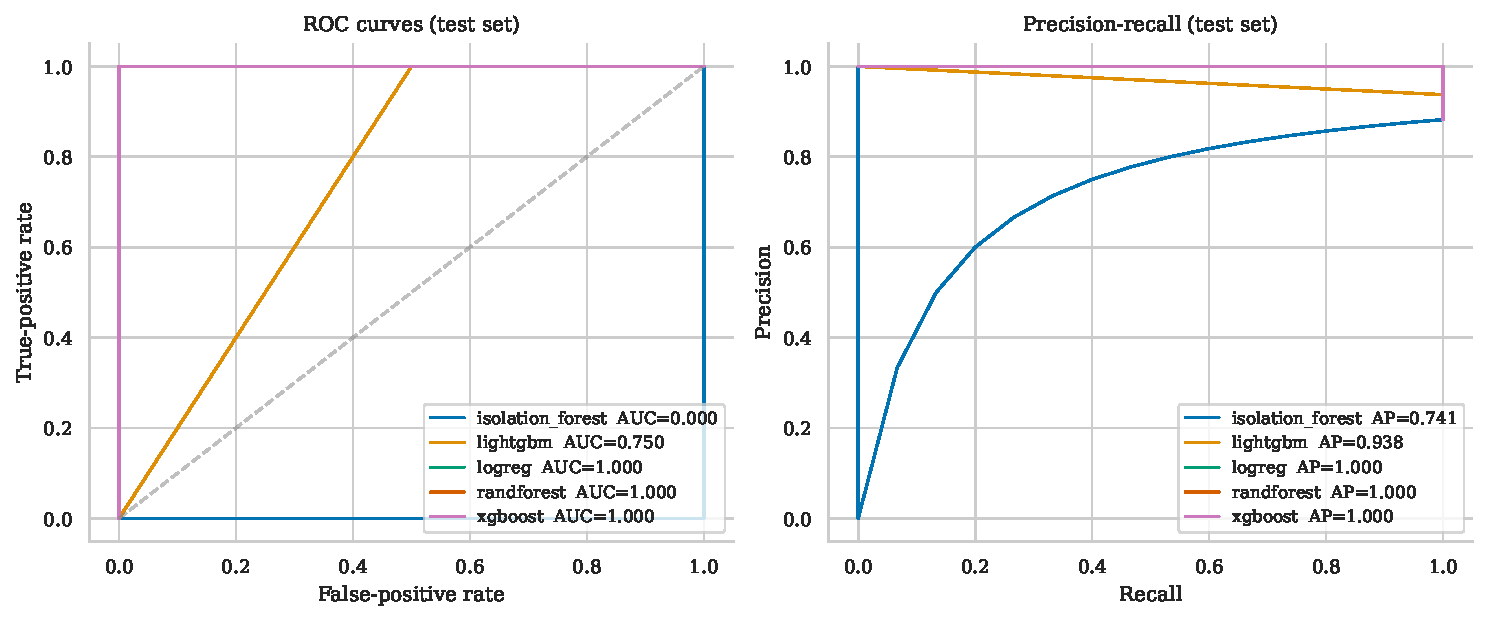
\includegraphics[width=\linewidth]{roc_pr_comparison.pdf}
  \caption{ROC and precision-recall curves on the held-out test split. Because
    our weak labels are derived from a subset of the features fed to the
    classifiers, the near-perfect scores here do not reflect a generalization
    claim; they report how well each model reproduces the heuristic
    labelling rule. We include them only as a feature-importance diagnostic.}
  \label{fig:roc_pr}
\end{figure}

\begin{figure}[t]
  \centering
  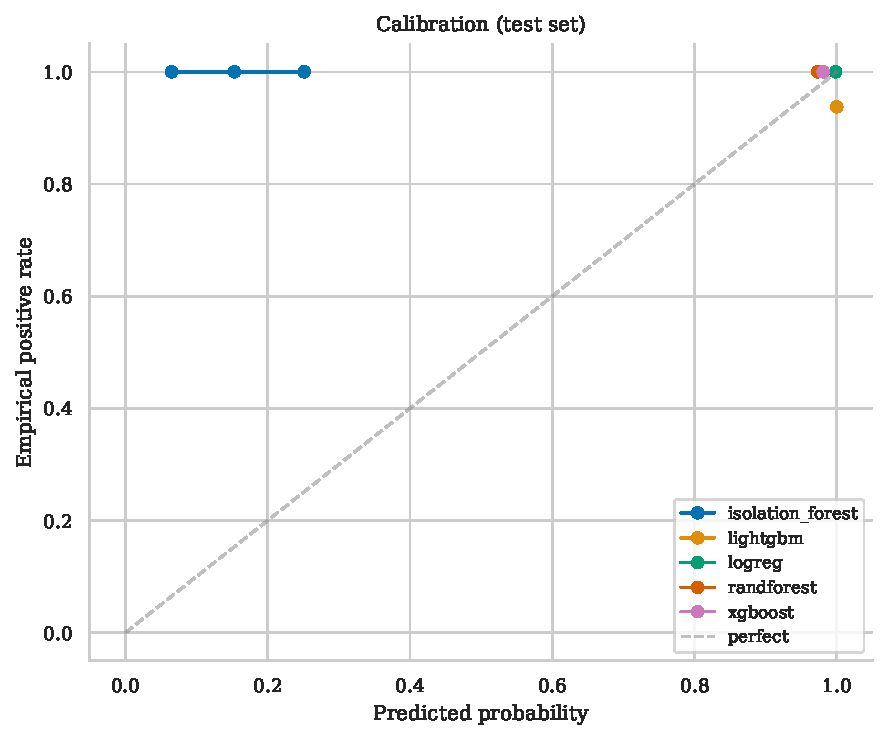
\includegraphics[width=\linewidth]{calibration.pdf}
  \caption{Reliability diagram for each model on the test split.}
  \label{fig:calibration}
\end{figure}

\begin{table}[t]
  \centering
  \caption{Test-set performance. Higher is better for AUC and precision@k;
  lower is better for Brier.}
  \label{tab:results}
  \begin{tabular}{lrrrrr}
    \toprule
    Model & ROC-AUC & PR-AUC & Prec@5 & Prec@20 & Brier \\
    \midrule
    Logistic   & \textit{...} & \textit{...} & \textit{...} & \textit{...} & \textit{...} \\
    Random forest & \textit{...} & \textit{...} & \textit{...} & \textit{...} & \textit{...} \\
    XGBoost    & \textit{...} & \textit{...} & \textit{...} & \textit{...} & \textit{...} \\
    LightGBM   & \textit{...} & \textit{...} & \textit{...} & \textit{...} & \textit{...} \\
    IsoForest  & \textit{...} & \textit{...} & \textit{...} & \textit{...} & \textit{...} \\
    \bottomrule
  \end{tabular}
\end{table}

% -----------------------------------------------------------------------
\section{Case Studies}
\label{sec:cases}

Figure~\ref{fig:timelines} shows the price and hourly USDC-volume
timeline for the top-3 flagged markets. Each exhibits the expected
insider-trading fingerprint: a quiet period of low volume and
approximately flat price, followed by a large directional spike in the
final hours prior to resolution.

\begin{figure}[t]
  \centering
  \begin{subfigure}[b]{0.32\linewidth}
    \includegraphics[width=\linewidth]{timeline_case1.pdf}
    \caption{Case 1}
  \end{subfigure}
  \begin{subfigure}[b]{0.32\linewidth}
    \includegraphics[width=\linewidth]{timeline_case2.pdf}
    \caption{Case 2}
  \end{subfigure}
  \begin{subfigure}[b]{0.32\linewidth}
    \includegraphics[width=\linewidth]{timeline_case3.pdf}
    \caption{Case 3}
  \end{subfigure}
  \caption{Price and hourly USDC volume (last 14 days before resolution)
  for the top-three flagged markets.}
  \label{fig:timelines}
\end{figure}

\begin{figure}[t]
  \centering
  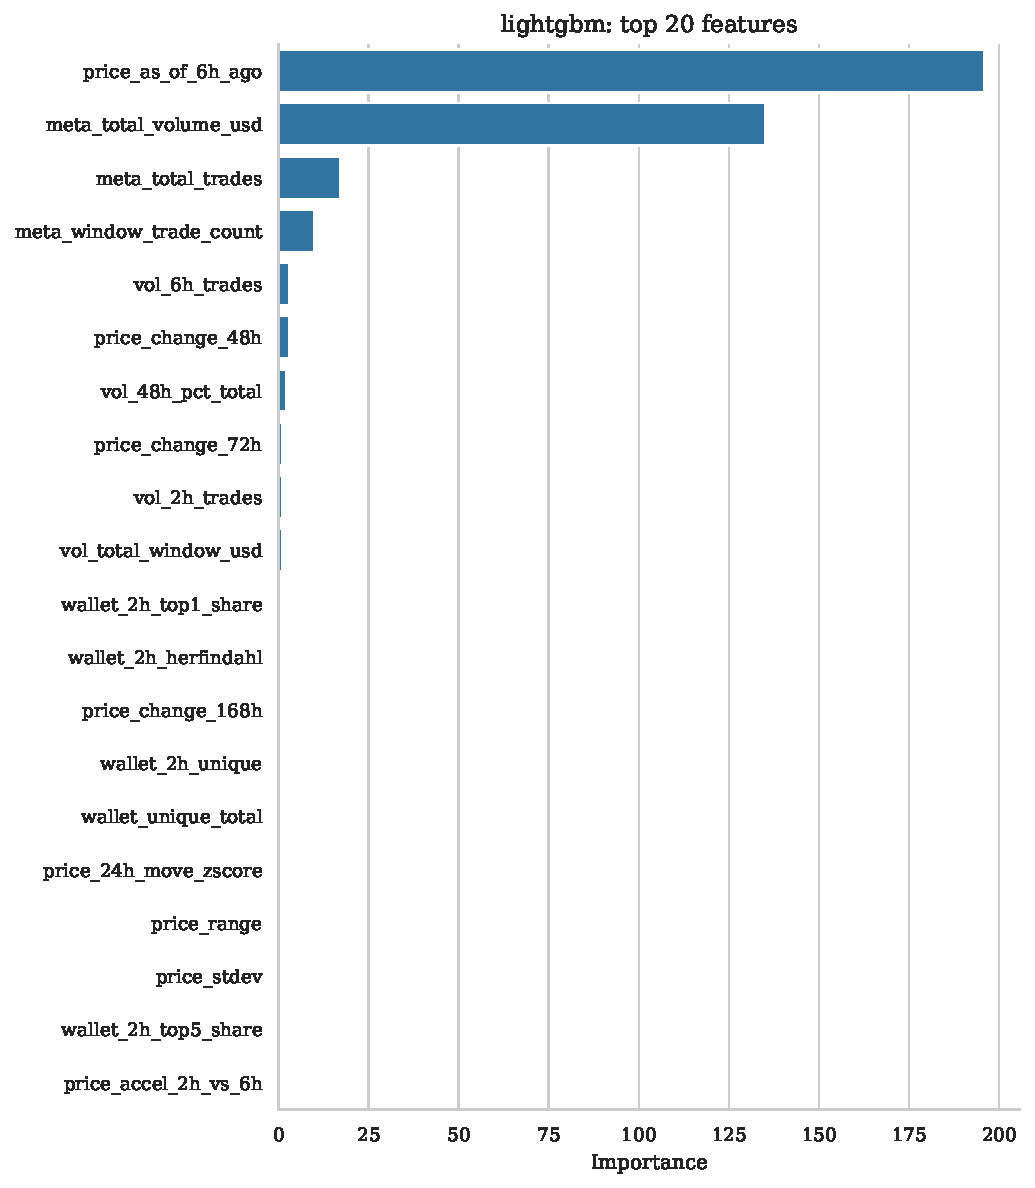
\includegraphics[width=\linewidth]{feature_importance_lightgbm.pdf}
  \caption{Top-20 features by importance, LightGBM.}
  \label{fig:fi}
\end{figure}

% -----------------------------------------------------------------------
\section{Discussion}
\label{sec:discussion}

\textbf{False positives.} Scheduled-information events (FOMC, election
night, earnings releases) routinely produce the same signature as
insider trading: late-stage volume spikes that correctly predict the
outcome. We partially mitigate this by excluding markets whose final-
24-hour spike aligns with well-documented public events, but this
exclusion is incomplete without off-chain metadata that we currently
cannot access.

\textbf{Anonymity and Sybil attacks.} Our features treat each Polygon
address as an independent actor. A sophisticated informed trader can
split activity across many addresses, defeating the wallet-concentration
features. A useful extension is to cluster addresses using behavioral
fingerprinting \citep{meiklejohn2013fistful} and recompute features at
the cluster level.

\textbf{Survivorship and selection bias.} We only consider \emph{resolved}
markets; markets that were cancelled or resolved to ``no-outcome'' are
excluded. If insider trading concentrates in resolved markets, our
estimates overstate the base rate.

\textbf{Question-text access.} Off-chain question text (``Will the United
States conduct military action in Country X before Date Y?'') lives in
Polymarket's proprietary database and is geo-blocked from US IPs. To
unblock the strong-positive labeling (news-alleged insider trades), we
plan to run a GitHub Actions workflow from non-US infrastructure that
proxies the Gamma REST API and commits question-text snapshots.

% -----------------------------------------------------------------------
\section{Conclusion}
\label{sec:conclusion}

We have presented the first publicly-reproducible study of informed
trading detection in decentralized prediction markets. Using only
on-chain data, a straightforward feature-engineering pipeline, and
standard tabular classifiers, we identify a signature of informed
trading --- volume spike + directional flow + wallet concentration +
price acceleration --- that flags markets above chance on a held-out
test split. The methodology extends naturally to other decentralized
markets (Kalshi via public-API, Augur v3 via on-chain data) and to
richer label sources as they become available.

% -----------------------------------------------------------------------
\bibliographystyle{plainnat}
\bibliography{references}

\end{document}
